\subsection*{Введение в классификацию}
Задача классификации кажется одной из самых естественных в машинном обучении: у нас есть объект с набором признаков, и нужно определить, к какому классу он относится. Это может быть письмо, которое либо является спамом, либо нет. Это может быть медицинская запись, где нужно понять, болен человек или здоров. Это может быть изображение, на котором может оказаться кошка, собака или что-то ещё.

Формально различают несколько видов классификации. Если классов всего два --- говорят о \textit{бинарной классификации}. Если классов больше, задача называется \textit{многоклассовой}. 

Целью последующих занятий является формальное определение задачи 
классификации, решение возникающих трудностей о которых далее),
а также вывод алгоритмов, которые способны решать данную задачу.

\subsection*{Постановка задачи классификации}

Итак, в задаче регрессии, постановка была в целом понятной "--- есть некоторая целевая переменная, которая может принимать любое значение на вещественной прямой. Задача модели "--- восстановить некоторую функцию, которая бы изящно описывала эти данные, и предсказывать целевую переменную на новых объектах с относительно небольшой погрешностью. То есть:
\[
\mathbb{Y} \in \mathbb{R}^d
\]

В случае классификации, ситуация сильно упрощается:
\[
\mathbb{Y} \in \{-1, +1\}
\]
Будем говорить, что $y = -1$ "--- \textit{отрицательный ответ}, 
а $y = +1$ "--- \textit{положительный ответ}.

То есть, у каждого объекта выборки в качестве целевой переменной 
выступает некоторый класс "--- является ли письмо спамом или нет, 
здоров ли текущий пациент или ему стоит полежать ещё немного и т.д.

Наша текущая задача "--- построить какую-нибудь простенькую модель, 
которая способна решать задачу классификации. Но сначала надо определить, что должна делать функция, которую мы собственно строим. Взгляните на следующее изображение:
\begin{figure}[H]
    \centering
    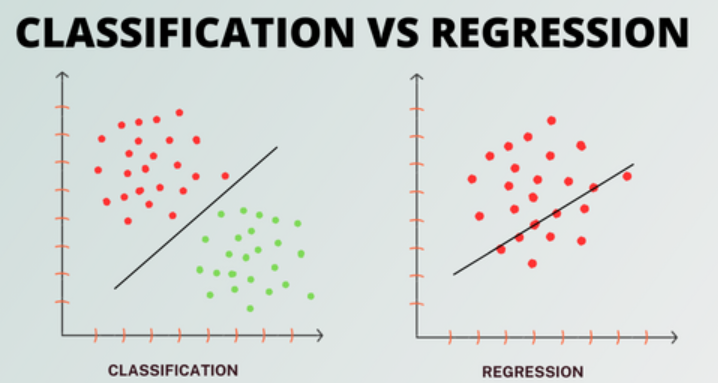
\includegraphics[width=0.75\linewidth]{media/regr_vs_class.png}
\end{figure}

Как мы видим, теперь нашей целью является построение такой прямой 
(гиперплоскости), которая будет в состоянии отделить один класс от другого.

Ну, давайте возьмём уже известную нам модель из задачи регрессии, и просто возьмём её знак:
\[
a(x) = sign(\langle w, x\rangle + b)
\]
Операция $sign$ возвращает 1 для положительных чисел и -1 для отрицательных. Как раз то, что нам нужно для нашей задачи.

Обучение зададим так:
\[
\frac {1}{\ell} \sum_{i=1}^\ell [sign(\langle w, x\rangle + b) \ne y_i] -> \min_w
\]

Квадратные скобки тут означают \textit{предикат}, т.е. если условие внутри них выполняется - возвращается 1, иначе 0. Соответственно мы считаем количество тех объектов, на которых классификатор сработал некорректно.

Эта функция потерь называется \texttt{error rate} (доля ошибок). Однако сразу же мы натыкаемся на следующую проблему: невозможность взять производную. Действительно, функция потерь является дискретной, и никакого изменения весов ожидаться не будет. Соответственно, единственный способ решить такую задачу "--- перебирать вектор весов до тех пор, пока нам не попадётся оптимальный. Задачи, которые решаются только перебором (т.е. нет оптимального алгоритма решения) называются \texttt{NP}"=полные задачи. Сейчас нам нужно придумать, как оптимально решать задачу обучения классификатора.

Чтобы исправить эту ситуацию, введём 
\[
M = y_i\langle w, x\rangle
\]
M "--- \texttt{margin}, или же отступ классификатора. 

Можно сказать, что \texttt{margin} - это уверенность классификатора. Если отступ маленький, т.е. объект находится близко к гиперплоскости, то при минимальном изменении весов класс на этом объекте может поменяться. В таких случаях говорят о неуверенности классификатора. Однако, как правило, если отступ сильно меньше 0, это обычно у выбросов.

Запишем следующую функцию потерь:
\[
L(M) = [M < 0]
\]
И выведем её график:
\begin{figure}[H]
    \centering
    
\includegraphics[width=0.75\linewidth]{media/margin.png}
\end{figure}

Тут всё та же проблема, что и в функции потерь выше: мы никак не сможем
посчитать градиент. Однако тут нам открывается интересная возможность "--- взять какую"=то функцию, которая будет похожа на $[M < 0]$, но при этом от неё будет реально взять производную.

Пример такой функции:
\[
\tilde{L}(M) = \exp^{-M}
\]

\begin{figure}[H]
    \centering
    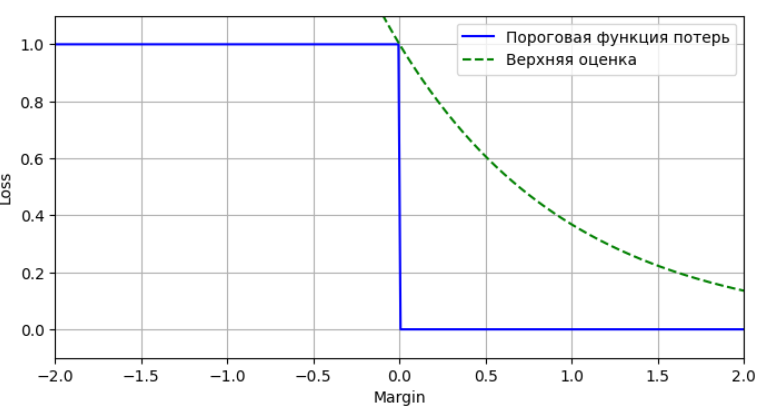
\includegraphics[width=0.75\linewidth]{media/margin_expr.png}
\end{figure}

Введённая функция называется \textit{верхней оценкой} функции $[M > 0]$. И соответственно, плясать мы будем от этого "--- вводить новые верхние оценки и обосновывать, почему они действительно имеют смысл.

На дальнейших занятиях мы рассмотрим:
\begin{enumerate}
    \item $\tilde{L}(M) = \log(1 + \exp^{-M})$ "--- логистическая функция потерь;
    \item $\tilde{L}(M) = \max(0, 1 - M)$ "--- метод опорных векторов.
\end{enumerate}